\chapter{Buck converter}
This lab follows the tutorial on the Buck converter, the statement of which is recalled below.
The objective is to use the LTSpice software to simulate the circuit and understand its operation.
LTSpice is software provided by Analog Device, based on Spice simulation. The software documentation is available on the Analog Device website: \href{https://www.analog.com/en/resources/design-tools-and-calculators/ltspice-simulator/ltspice-recommended-reading-list.html}{Analog Device Website}

We want to power an STM32H4 microprocessor using a battery. The specifications are as follows:

\begin{itemize}
\item LiPo 2S battery $V_{in} = 7.4\ V$
\item Microprocessor supply voltage: $V_{out}=3.3\ V$
\item Maximum input voltage ripple for the microprocessor: $\Delta V_S = 50\ mV$
\item Nominal output current: $I_S = 200\ mA$
\item Current ripple: 30\%
\end{itemize}

For this, we want to use the following component: \textbf{LT1959}, an excerpt from the documentation is in the appendix.
In this exercise, we will assume that the \underline{\textbf{components are}} \underline{\textbf{perfect}}, and that the Buck operates in \underline{\textbf{continuous conduction mode}}.

\section{Preparation}

\begin{enumerate}
\item Draw the circuit to use this component in Buck operation
\item Recall the values of (no calculation is required):
\begin{itemize}
    \item the switching frequency of the converter
    \item the values of $L_1$, $C_1$ for the output filter of the converter to meet the specifications
    \item the feedback resistances $R_1$ and $R_2$ to achieve an output voltage of $3.3\ V$
    \item the value of the resistance $R_m$ modeling the microcontroller drawing a nominal current
    \item the values of $R$ and $C$ for the output voltage control, limiting the duty cycle at startup to $\dfrac{\alpha_n}{2}$ and a time constant of the controller 10 times higher than the time constant of the uncorrected system
\end{itemize}
\end{enumerate}

\newpage
\section{Circuit Simulation}

Here is a brief summary of the LTSpice interface. For more information, you can refer to the Analog Device page:
\href{https://www.analog.com/en/resources/design-tools-and-calculators/ltspice-simulator/ltspice-recommended-reading-list.html}{Analog Device Website}

\begin{figure}[h]
    \centering
    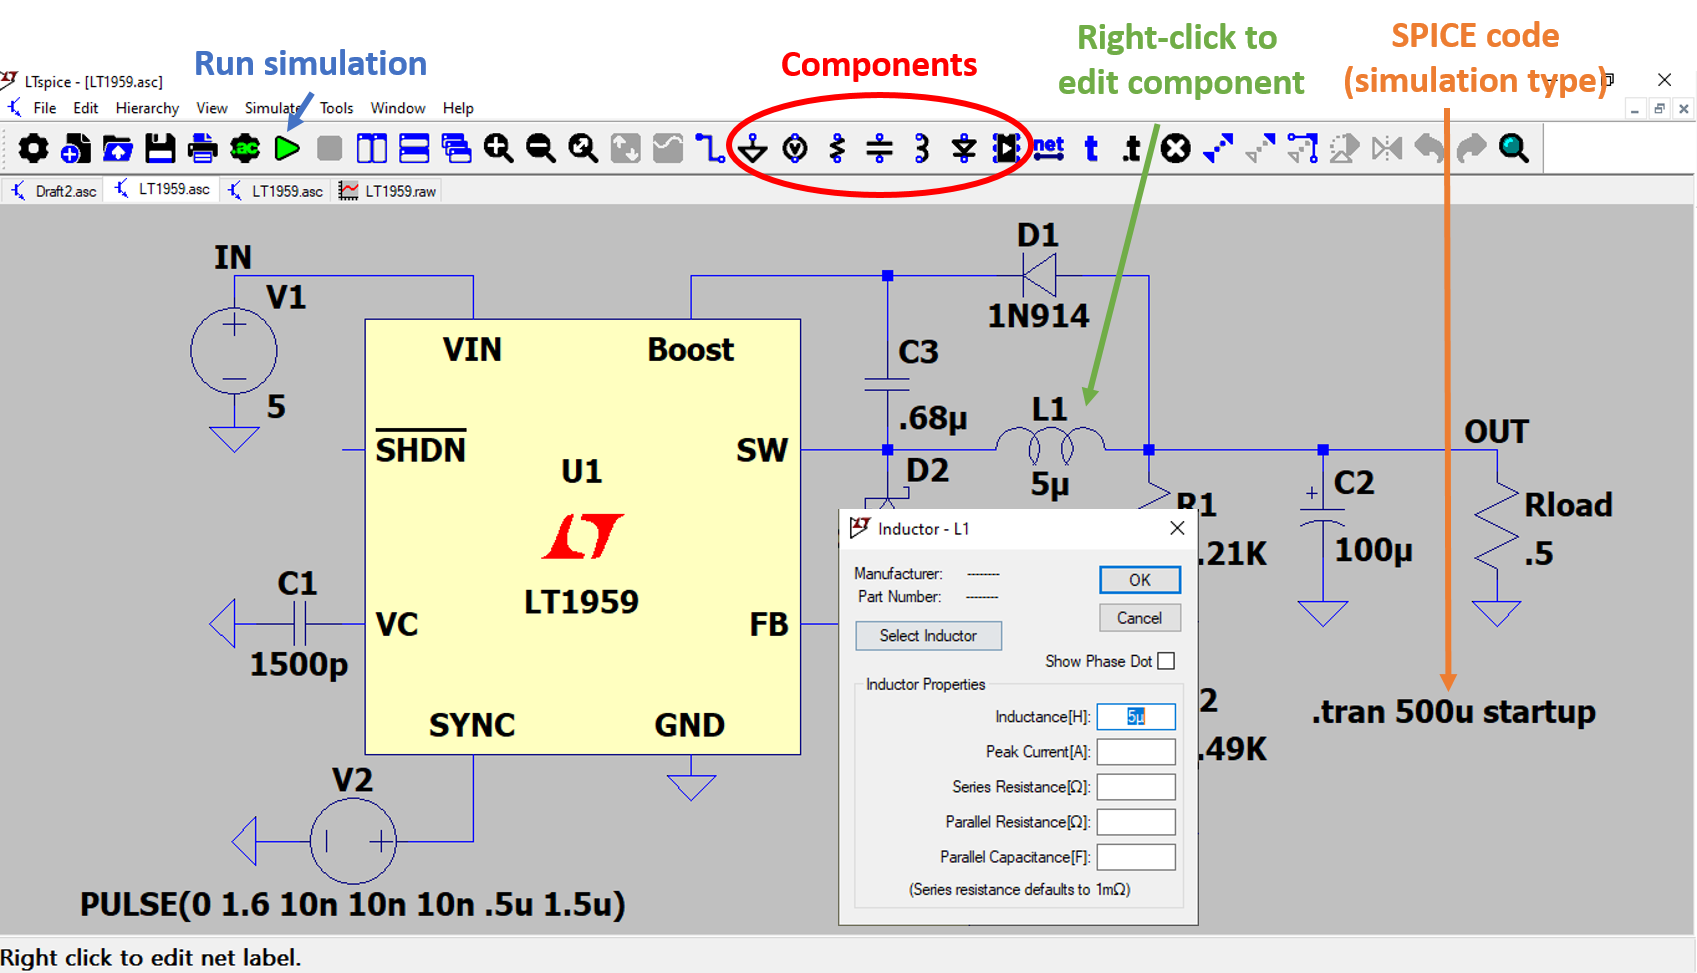
\includegraphics[width=\linewidth]{TP_Buck/fig/LTSpice.png}
\end{figure}

\begin{itemize}
\item Create a new \textit{Schematic} and place the \textbf{LT1959}.
\item Create the circuit from the datasheet by right-clicking on the component $\Rightarrow$ "\textit{Open Example Circuit}"
\item Modify the circuit to match the datasheet. The "\textit{SYNC}" pin will not be used.
\item Adjust the component values to meet the specifications.
\item Perform a transient simulation. To do this, go to "\textit{Simulate}" $\Rightarrow$ "\textit{Configure Analysis}" $\Rightarrow$ "\textit{Transient}" and run a simulation for 3 ms.
\end{itemize}

\begin{enumerate}
\item Verify the switching frequency of the converter
\item Verify that the specifications are met: output voltage, current ripple, voltage ripple
\item Does the converter operate in continuous or discontinuous conduction mode?
\end{enumerate}

\section{Component Influence}

\begin{enumerate}
    \item Measure the current ripple in $L_1$ and the output voltage ripple for different values of $L_1$. Comment.
    \item Measure the output voltage ripple for different values of $C_1$. Comment.
    \item Determine the value of $L_1$ for critical conduction mode. Verify by simulation.
\end{enumerate}

\section{System Speed and Stability}

\begin{enumerate}
    \item Modify the value of $C$ and measure the 5\% response time. Comment.
    \item By modifying the value of $R$, determine the maximum resistance value at which the system becomes unstable.
    \item Add a current generator in parallel with the resistance $R_s$ to generate a current pulse (once the system is in steady state). This pulse can model a sudden current demand from the system powered by the Buck. Determine the new value of $R$ at which the system becomes unstable during a disturbance.
\end{enumerate}